\chapter{Data}
\label{app:data}

\section{Income Surveys}

Measures of income are drawn from two principal data sources, both provided by the ABS. The first is the Survey of Income and Housing, a detailed sample survey of household income dynamics, and the second is the Census of Population and Housing, a five-yearly survey of the full Australian population. 

\subsection{Survey of Income and Housing, 1981-2012}
\label{sec:SIH}

% \cite{ATKINSON2007} - under-estimate top income earners

The Survey of Income and Housing (SIH) is a hierarchical, clustered sample survey of income and expenditure patterns of the the Australian population, periodically conducted by the Australian Bureau of Statistics. It was first conducted in the 1981-2 fiscal year, followed by 1985-6, and then every two or three years from 1994-5. Microdata files were obtained as confidentialized unit record files (CURFs) for the surveys performed in 1981-2, 1985-6, 1994-5, 1995-6, 1996-7, 1997-8, 2000-1, 2002-3, 2005-6, 2007-8 and 2009-10.

Unlike the Census of Population and Housing, a population survey, the SIH is conducted on just a sample of the population, and unit records are weighted by demographic variables in order to create a representative sample. Weights are produced at three levels of the survey hierarchy: household, income unit and person. (In addition, the SIH is occasionally produced simultaneously with the Housing Expenditure Survey, or HES, in which case further expenditure levels are recorded.) For the purposes of this project, only individual-level records are of interest, and so all estimators are weighted by person weight.

\subsubsection{Survey Weights}

In all versions of the SIH, the $PERS\_WT$ variable for the $i$th record is computed as the reciprocal of that individual's probability of selection $\pi_i$, where $PERS\_WT_i = 1/\pi_i.$ $PERS\_WT_i$ can be interpreted as the number of individuals in the whole population `represented' by record $i$. The sum of the inverse selection probabilities is therefore identically equal to the size of the population. Note that, since the $\pi_i$ refers to the probability of individual $i$ being drawn from the overall population (and not from the sample), the selection probabilities $\pi_i$, $i=1,\cdots,n$, will not sum to 1.



\subsubsection{Occupational Coding Schemes}
\label{sec:occcoding}

In major surveys such as the SIH and Census, respondents' occupations are coded according to standard occupational classification schemes. One major drawback of the SIH is that, over its 30 year history, several distinct and incompatible occupational coding schemes have been used. In particular, the classification schemes for the available editions of the survey are:
\begin{enumerate}
\item 1981/82: occupations are coded using the CCLO.
\item 1985/86, 1994/95: occupations are coded using ASCO version 1, at the major group level.
\item 1995/96 to 1997/98: occupations are coded using ASCO version 2, at the major group level.
\item 2000/01 to 2002/03: occupations are coded using ASCO version 2, at the minor group level.
\item 2007/8 to 2011/12: occupations are coded using ANZSCO, at the minor group level.
\end{enumerate}
Revisions to occupational classification schemes are conducted from time to time by statistics bureaus in response to changing reporting requirements, and also to keep with changes in the composition of the work force over time. As new schemes are introduced, such as the ASCO II \citep{Castles1986} and the ANZSCO \citep{Trewin2006}, link tables are usually produced in order to convert statistical data tabulated using the previous coding scheme to the new scheme. Indeed, detailed link tables are available for both the ANZSCO and ASCO II, and provide a detailed mapping between both schemes. Unfortunately, however, link tables are generally constructed at the finest-grained level of the occupational classfication. In the case of the ANZSCO and both editions of the ASCO, occupational groupings at the minor group (two-digit) level cannot be cleanly mapped from one classification scheme to the other. One occupational group in the ANZSCO might map to several occupational groups in the ASCO II, and vice-versa.

One solution to the problem of incompatible groupings is to create a hybrid classification scheme by pooling occupational super-groups. Although this approach is not perfect---occupational groupings are complex, and a perfect hybrid classification scheme is unlikely to be possible---it does allow a good approximate comparison of occupational wage profiles over time. In this project, a comparison was required between two pairs of periods: 1981/82 and 2011/12 and 2000/01 and 2011/12. Unfortunately, the CCLO, ASCO II and ANZSCO are all sufficiently different, that a hybrid scheme that could accommodate all three periods would have to include very few, very large groups of occupations, reducing the sensitivity of the analysis considerably. Therefore, two schemes were designed, {\tt COMBINEDI} for comparing 1981/82 and 2011/12 (Table~\ref{tab:combined1}), and {\tt COMBINEDII} for comparing 2000/01 and 2011/12 (Table~\ref{tab:combined2}). One advantage of maintaining two separate hybrid classification schemes, is that the different schemes serve as an empirical check on the analysis procedure. Despite the different aggregation schemes, similar results should be obtained from both schemes.

The schemes were manually compiled using an iterative procedure. First, fine-grained occupations which comprise each occupational group code in each classification scheme were obtained from \citep{Castles1986} and \citep{Trewin2006}. Then, the corresponding occupational group in the other scheme was identified, by going through its occupations. If a group in one scheme mapped to multiple groups in the other, then the groups were deemed to be inseperable, and were merged together in the hybrid classification. Records with no or unknown occupations were simply dropped, as were occupations within the armed forces.

\begin{sidewaystable}[ht]
\centering
\begin{tabular}{clll}
  \hline
{\bf Group} & {\bf Occupation Title} & {\bf CCLO Codes} & {\bf ANZSCO Codes} \\ 
  \hline
   1 & Other managers & 12 & 10, 13, 22, 51 \\ 
   2 & CEOs, general managers, Legislators & 2 & 11 \\ 
   3 & Health professionals & 3--5 & 25, 41 \\ 
   4 & Professionals NFD & 10 & 20, 26 \\ 
   5 & Teachers & 6 & 24 \\ 
   6 & Legal Professionals & 7 & 6 \\ 
   7 & Designers, Engineers, Scientists, Transport Professionals & 1, 2, 23, 37 & 23 \\ 
   8 & Technicians & 9 & 30, 31 \\ 
   9 & Road transport \& railway workers & 24, 28-30, 32 & 73 \\ 
  10 & Electrotechnology and Telecommunications trades workers & 31,39 & 34 \\ 
  11 & Office support, clerical and postal workers & 14, 15, 25, 26 & 50, 52--56, 59  \\ 
  12 & Farmers/farm managers & 19 & 12 \\ 
  13 & Farm/rural/garden workers & 20, 21 & 84 \\ 
  14 & Storepersons, freight handlers & 50 & 74 \\ 
  15 & Labourers & 51 & 80, 82, 89 \\ 
  16 & Construction trades workers & 41, 43 & 33 \\ 
  17 & Food trades workers & 45 & 35, 85 \\ 
  18 & Arts and media professionals & 8, 42, 59 & 21 \\ 
  19 & Hospitality workers & 54 & 14, 43 \\ 
  20 & Other technicians and trades workers & 33--35, 44, 46, 47, 56 & 36, 39 \\ 
  21 & Sales representatives and agents & 16, 17 & 61 \\ 
  22 & Sales assistants and support workers & 13, 18 & 60, 62, 63 \\ 
  23 & Automotive and Engineering trades workers & 36, 38, 40 & 32 \\ 
  24 & Cleaners and caretakers & 53, 55, 57 & 42, 81 \\ 
  25 & Sports and personal service workers & 58, 60 & 40, 45 \\ 
  26 & Factory process workers & 48 & 83 \\ 
  27 & Protective service workers & 52 & 44 \\ 
  28 & Machine operators & 49 & 70, 71, 72 \\ 
   \hline
\end{tabular}
\caption{The {\tt COMBINEDI} mapping, at the two-digit level, between the 1976 Census Classification and Classified List of Occupations (CCLO) and the 2006 Australian and New Zealand Standard Classification of Occupations (ANZSCO). This classification is used to compare the 2000/01 and 2011/12 ABS surveys of income and housing.}
\label{tab:combined1}
\end{sidewaystable}

\begin{sidewaystable}[ht]
\centering
\begin{tabular}{clll}
  \hline
{\bf Group} & {\bf Hybrid Occupation Group Title} & {\bf ASCO II Codes} & {\bf ANZSCO Codes} \\ 
  \hline
  1 & General Managers, Legislators & 10, 11 & 10, 11 \\ 
  2 & Farm Managers & 13 & 12 \\ 
  3 & Specialist Managers & 12 & 13 \\ 
  4 & Hospitality and Service Managers and Workers & 33 & 14 \\ 
  5 & Other Professionals & 20 & 20, 21 \\ 
  6 & Business, ICT Professionals & 22 & 22, 26 \\ 
  7 & STEM Professionals & 21 & 23 \\ 
  8 & Education Professionals & 8 & 24 \\ 
  9 & Health Professionals & 9 & 25 \\ 
  10 & Sales supervisors and agents & 40, 49 & 61 \\ 
  11 & Legal Professionals & 25 & 27 \\ 
  12 & Technicians & 31 & 30, 31 \\ 
  13 & Auto and engineering tradespersons & 41, 42 & 32 \\ 
  14 & Construction tradesworkers & 44 & 33 \\ 
  15 & Electricians and telecom tradesworkers & 43 & 34 \\ 
  16 & Food trades workers & 45 & 35 \\ 
  17 & Skilled Animal and Horticultural Workers & 46 & 36 \\ 
  18 & Associate Professionals & 30, 39, 63, 83 & 39, 44, 45 \\ 
  19 & Clerical Workers & 50, 60, 61, 81 & 50, 53--56 \\ 
  20 & Business and Administration Associate Professionals & 32 & 42, 51 \\ 
  21 & Personal Assistants and Secretaries & 51 & 52 \\ 
  22 & Other Clerical and Administrative Workers & 59 & 59 \\ 
  23 & Sales workers & 80, 82 & 60, 62, 63 \\ 
  24 & Plant operators & 70 & 70, 71, 72 \\ 
  25 & Road and rail drivers & 70--72 & 73 \\ 
  26 & Other production workers & 79 & 74, 83 \\ 
  27 & Labourers & 90,92,99 & 80, 82, 84, 85, 89 \\ 
  28 & Cleaners & 91 & 81 \\ 
  29 & Health and Welfare Support Workers & 34 & 40, 41 \\ 
   \hline
\end{tabular}
\caption{The {\tt COMBINEDII} mapping, at the two-digit level, between the 1996 Australian Standard Classification of Occupations, 2nd Edition (ASCO II) and the 2006 Australian and New Zealand Standard Classification of Occupations (ANZSCO). This classification is used to compare the 1981/82 and 2011/12 ABS surveys of income and housing.}
\label{tab:combined2}
\end{sidewaystable}

\subsubsection{Educational Attainment}


\subsubsection{Sources of Income}

As described in the data appendix, to ensure comparability for skills, only individuals who report a full-time wage as their primary source of income are included. (** NB: later we might attempt \$ per hour)



\subsection{Census}

\section{Occupational Data}
\label{sec:occclassify}

One step which was skipped over in the informal analysis in the previous chapter was the assignment of occupations into task groups, on the basis of the occupational classification scheme. If task content is to be analyzed rigorously, and in greater detail than a simple three-occupation breakdown, a quantitative view of occupational task content is required. 

\subsection{Australia \& New Zealand Standard Classification for Occupations (ANZSCO)}

The standard classification scheme for occupations used in Australia, ANZSCO, simply lists by name the tasks a particular job title might be required to perform. These tasks are listed in an occupation-specific way, such that they cannot be compared between occupations. For example, under the unit group 2243: {\em Economists}, the required tasks include
\begin{quote}
{\em Analysing interrelationships between economic variables and studying the effects of government fiscal and monetary policies, expenditure, taxation and other budgetary policies on the economy and the community \citep[p.185]{Trewin2006}}
\end{quote}

{\em Statisticians} (unit group 2441) perform tasks that are largely similar to that of economists, even though the underlying theory that motivates their work may be somewhat different. A corresponding task entry for statisticians includes
\begin{quote}
{\em Defining, analysing and solving complex financial and business problems relating to areas such as insurance premiums, annuities, superannuation funds, pensions and dividends \citep[p.181]{Trewin2006}}
\end{quote}
Given the qualitative nature of this classification scheme, there is no obvious way to systematically formalise the similarity between economists and statisticians on the basis of the ANZSCO classification. However, alternative classification schemes do exist which include comparable task classifications.

\subsection{Occupational tasks: O*NET}\label{sec:onet}

The U.S. equivalent to the ANZSCO classification, the O*NET database, includes hundreds of quantitative scales for the level of work activities, knowledge types and abilities for individuals in each of approximately five hundred occupations. The data were constructed using expert surveys, and provide a very rich source of information about the activities that workers in each occupation actually undertake. For example, for the work activity {\em analyze data}, the occupations {\em economist} and {\em surgeon} score highly (6.58/7 and 5.49/7, respectively.) But for the work activity {\em Handle moving objects}, surgeons score 3.62/7, and economists score only 0.54/7.

We have mapped the ANZSCO (and its predecessors, various editions of ASCO and the CCLO) to the O*NET data, and sucessfully constructued a skill measure series for Australian occupational classification schemes. We then apply a transformation step, described by \citet{Firpo2011}, to build composite indexes for `automation,' `offshorability', and so on. These composite indexes provide a dependent variable which, along with levels of capital investment on an industry-by-industry basis, provide a basis by which changes in the occupational wage structure can be analyzed. The following five composite indexes are constructed for each occupation code:


\begin{enumerate}[A.]
\item Characteristics linked to Technological Change/Offshorability
\begin{enumerate}[1.]
\item Information Content 
  \begin{itemize}
  \item 4.A.1.a.1 Getting Information (JK)
  \item 4.A.2.a.2 Processing Information (JK) 
  \item 4.A.2.a.4 Analyzing Data or Information (JK) 
  \item 4.A.3.b.1 Interacting With Computers (JK) 
  \item 4.A.3.b.6 Documenting/Recording Information (JK)
  \end{itemize}
\item Automation/Routinization 
  \begin{itemize}
  \item 4.C.3.b.2 Degree of Automation 
  \item 4.C.3.b.7 Importance of Repeating Same Tasks 
  \item 4.C.3.b.8 Structured versus Unstructured Work (reverse) 
  \item 4.C.3.d.3 Pace Determined by Speed of Equipment 
  \item 4.C.2.d.1.i Spend Time Making Repetitive Motions
  \end{itemize}
\end{enumerate}
\item Characteristics linked to Non-Offshorability 
\begin{enumerate}[1.]
\item Face-to-Face
\begin{itemize}
  \item 4.C.1.a.2.l Face-to-Face Discussions 
  \item 4.A.4.a.4 Establishing and Maintaining Interpersonal Relationships (JK,B)
  \item 4.A.4.a.5 Assisting and Caring for Others (JK,B) 
  \item 4.A.4.a.8 Performing for or Working Directly with the Public (JK,B) 
  \item 4.A.4.b.5 Coaching and Developing Others (B)
\end{itemize}
\item On-Site Job 
\begin{itemize}
  \item 4.A.1.b.2 Inspecting Equipment, Structures, or Material (JK) 
  \item 4.A.3.a.2 Handling and Moving Objects 
  \item 4.A.3.a.3 Controlling Machines and Processes 
  \item 4.A.3.a.4 Operating Vehicles, Mechanized Devices, or Equipment 
  \item 4.A.3.b.4 Repairing and Maintaining Mechanical Equipment (*0.5) 
  \item 4.A.3.b.5 Repairing and Maintaining Electronic Equipment (*0.5)
\end{itemize}
\item Decision-Making 
\begin{itemize}
\item 4.A.2.b.1 Making Decisions and Solving Problems (JK) 
\item 4.A.2.b.2 Thinking Creatively (JK) 
\item 4.A.2.b.4 Developing Objectives and Strategies 
\item 4.C.1.c.2 Responsibility for Outcomes and Results 
\item 4.C.3.a.2.b Frequency of Decision Making
\end{itemize}
\end{enumerate}
\end{enumerate}

\begin{figure}
  \centering
  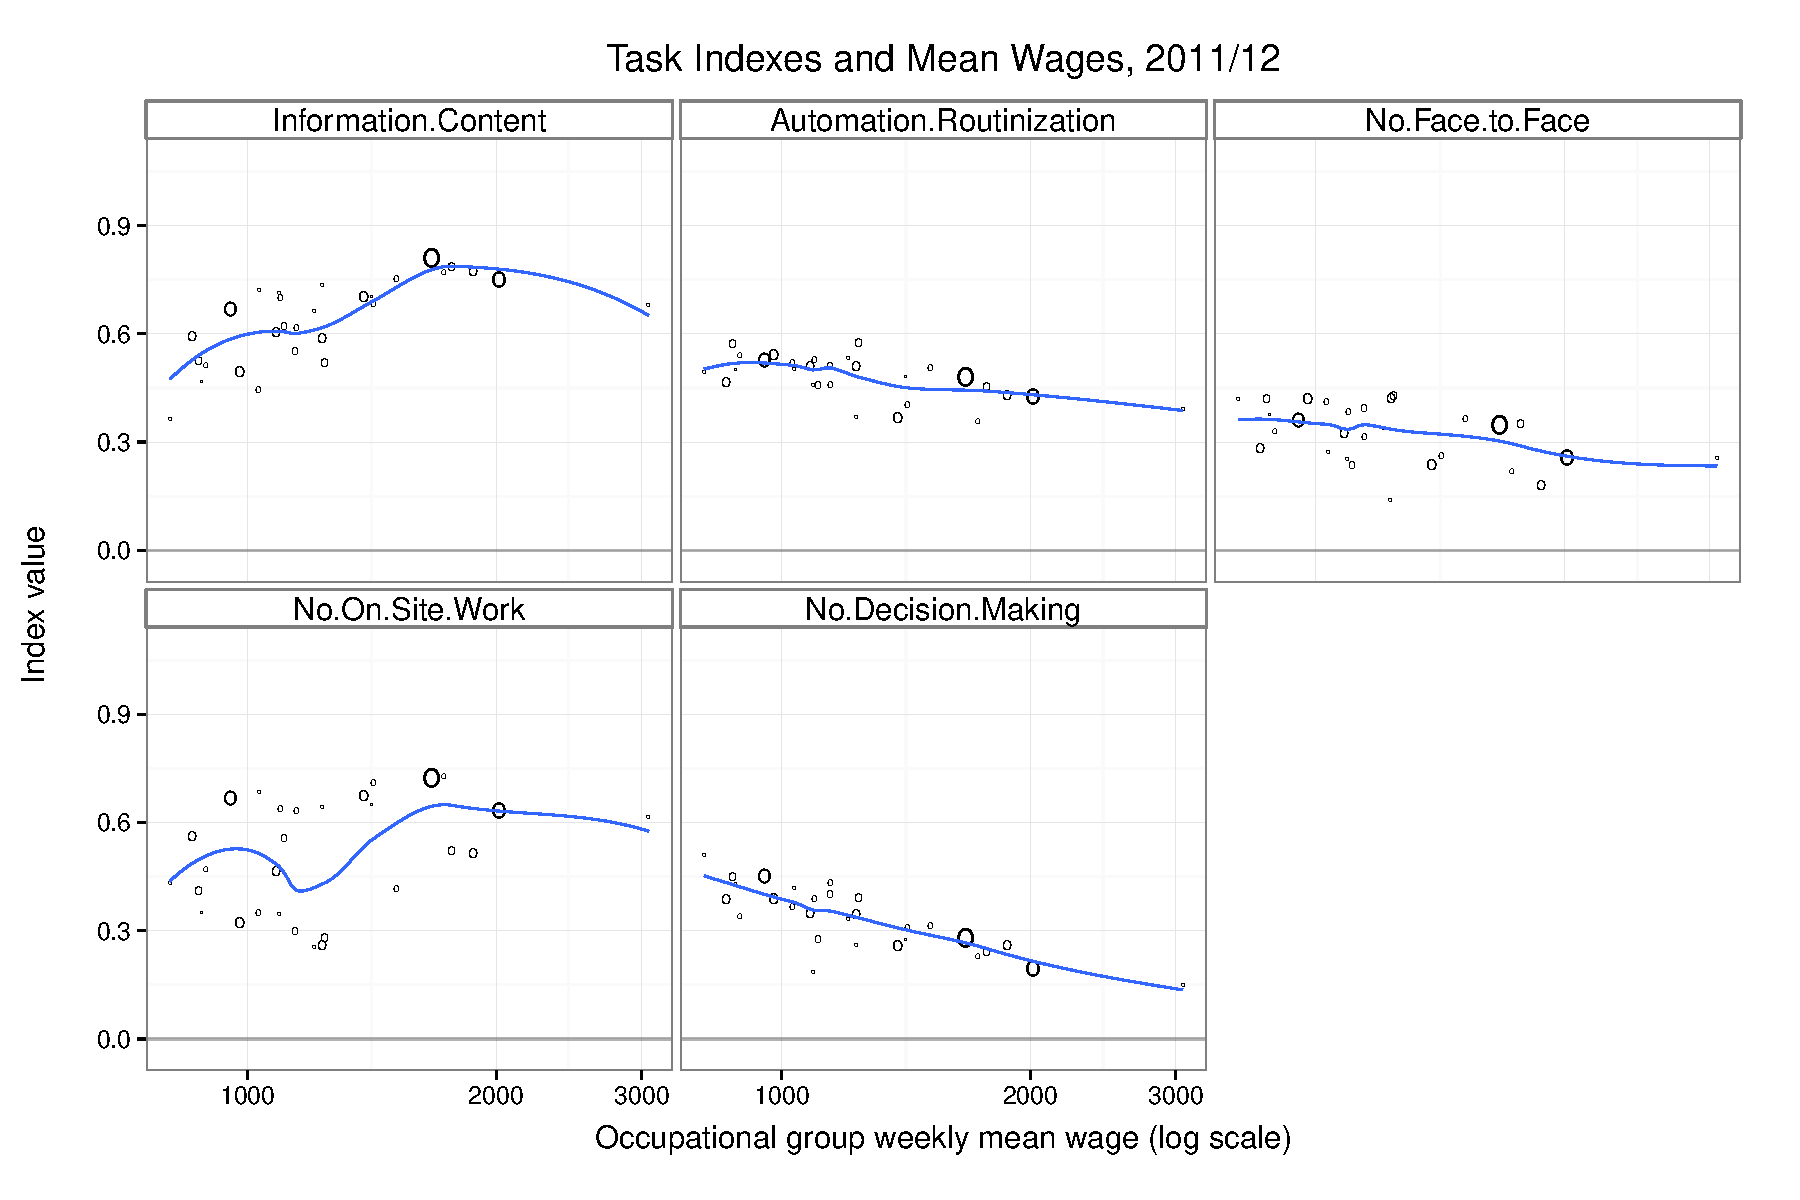
\includegraphics[width=\textwidth]{../figure/wages_indexes.pdf}
  \caption{Mean occupational wage and task measure index values, using second combined grouping. Note the similarity of the observed trend to Figure~\ref{fig:meanocc4dig}, in which occupations have not been grouped. Census respondents reporting full-time work are shown. The loess regression line is weighted by population; circle areas are proportional to population for each occupation. Sources: ABS cat 2072.0, O*NET, US Dept of Labor.}
  \label{fig:meanocc2}
\end{figure}

\begin{figure}
  \centering
  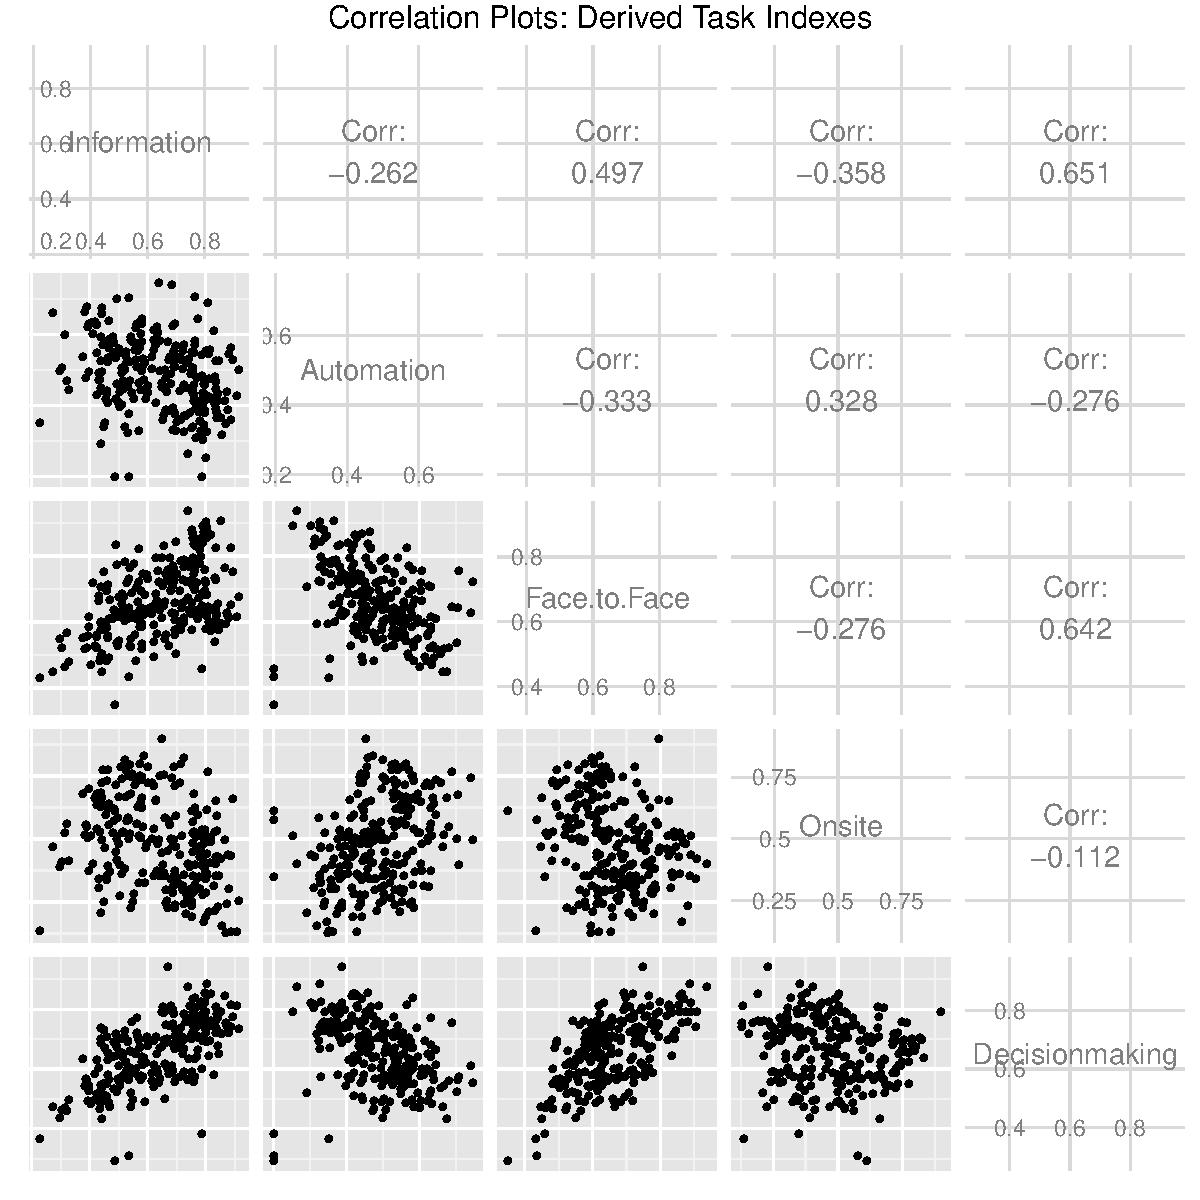
\includegraphics[width=\textwidth]{../figure/correl.pdf}
  \caption{Correlation plots: occupational task indexes for jobs at the ANZSIC 3-digit level. Notice that the job indexes are not perfectly mutually independent. As might be expected, `information content' is positively correlated with `face-to-face' roles ($\rho=0.497$) and decision-making ($\rho=0.651$), but negatively correlated with the job requiring on-site presence ($\rho=-0.358$). `Routinization' is negatively correlated with both face-to-face contact ($\rho=-0.33$) and decision-making ($\rho=-0.276$).}
  \label{fig:correl}
\end{figure}

%%% Local Variables: 
%%% mode: latex
%%% TeX-master: "paper"
%%% End: 
